\section{Coresets}

\begin{definition}
    Let $X \in \mathbb{R}^{n \times d}$, $y \in \{-1, 1\}^n$ be an
    instance of probit regression with sample weights
    $w \in \mathbb{R}^n_{>0}$ and let $z_i = -y_ix_i^T, \ i=1,...,n$.
    Then $C \in \mathbb{R}^{k \times d}$ weighted
    by $u \in \mathbb{R}^k_{>0}$ is a $(1 \pm \epsilon)$-coreset
    of $X$, $y$ for probit regression if
    \begin{equation*}
        \ (1 - \epsilon)f_{w, Z}(\beta)
        \leq f_{u, C}(\beta) \leq (1 + \epsilon)f_{w, Z}(\beta)
        \quad \forall \beta \in \mathbb{R}^d,
    \end{equation*}
    where $f_{w, Z}(\beta) = \sum_{i=1}^n w_i g(z_i \beta)$,
    $f_{u, C}(\beta) = \sum_{i=1}^k u_i g(c_i \beta)$ and
    $g(z) = -\log{\Phi(-z)}$.
\end{definition}

\subsection{Lower Bounds}

\begin{theorem}
    Let $X \in \mathbb{R}^{n \times 2}$, $y \in \{-1, 1\}^n$ be
    an instance of probit regression.
    Any coreset $C \in \mathbb{R}^{k \times 2}$ of $X$, $y$
    for probit regression consists of
    at least $k \in \Omega\left(\frac{n}{\log{n}}\right)$ points.
\end{theorem}
\begin{proof}
    We first show how such a coreset could be used in a
    communication protocol for the INDEX communication game
    to encode a message.
    Since there exists a lower bound on the minimum
    message length of the INDEX game (see~\cite{index}),
    we can use it to derive a lower bound on the
    coreset size.
    The same technique was also used in~\cite{on-coresets} to find
    lower bounds for coresets of logistic regression and is here slightly
    adapted for probit regression.

    The INDEX game consists of two players, Alice and Bob.
    Alice is given a random binary string $x \in \{0, 1\}^n$ of $n$ bits
    and Bob is given an index $i \in [n]$.
    The goal is for Alice to send a message to Bob that allows
    Bob to obtain the value $x_i$ of Alice's binary string $x$.
    It was shown in~\cite{index}, that the minimum length of a message
    sent by Alice that still allows Bob to obtain $x_i$ with
    constant probability is in $\Omega(n)$ bits.
    We will now see how a coreset for probit regression can be used
    to encode such a message.

    The first step is for Alice to convert her binary string $x$ into
    a set $P$ of two-dimensional points as follows:
    For each entry $x_j$ of her binary string where $x_j = 1$, she adds
    a point $p_j = \left( \cos{\left(2 \pi \frac{j}{n}\right)},
        \sin{\left(2 \pi \frac{j}{n}\right)} \right)$
    to her set $P$ and labels it with $1$.
    As we can see, all of these points are on the unit circle and all
    of them are labeled with $1$.
    Next, she uses these points to construct a coreset for probit regression
    $C \in \mathbb{R}^{k \times 2}$ of $P$
    and sends it to Bob. We will later see, how
    large the size $k$ of this coreset must be, so that Bob can still
    obtain $x_i$ with constant probability.

    As soon as Alice's coreset $C$ arrives at Bob, Bob can use it to
    obtain the value of $x_i$.
    To do this, Bob first adds two new points
    $q_1 = \left( \cos{\left(2 \pi \frac{i - 0.5}{n}\right)},
        \sin{\left(2 \pi \frac{i - 0.5}{n}\right)} \right)$
    and
    $q_2 = \left( \cos{\left(2 \pi \frac{i + 0.5}{n}\right)},
        \sin{\left(2 \pi \frac{i + 0.5}{n}\right)} \right)$
    to the set and labels both points with $-1$ (see figure~\ref{fig:index}).
    Next, he uses his points $q_1$ and $q_2$ together with the coreset $C$ to
    obtain a solution for the corresponding probit regression problem.
    He can then use the value of the cost function to determine the value
    of $x_i$ like this:

    Since Alice only added a point $p_j$ to her set if $x_j = 1$, both
    of his points $q_1$ and $q_2$ are linearly seperable from Alice's points if
    the value of $x_i = 0$, i.e. Alice didn't add a point for $x_i$.
    In this case, the value of the cost function tends to zero.
    If, on the other hand, Bob's new points $q_1$ and $q_2$ can't be linearly
    seperated from the other points, it means that Alice added a point
    for $x_i = 1$. In this case, there must be at least one
    misclassification and the value of the cost function is at least
    $g(0) = \log(2)$.
    Since coresets can be used to obtain $(1 + \epsilon)$-approximation
    of the objective function, Bob can use this case distinction to
    determine the value of $x_i$.

    There is one special case that has to be dealt with in order for this
    protocol to work. If Alice's coreset only consists of the single point
    $p_i$, Bob's points $q_1$ and $q_2$ could still be linearly seperated
    although Alice added $p_i$.
    The workaround to this is simple though:
    Bob can always just add two more
    points at the locations of $p_{i-1}$ and $p_{i+1}$ and label them with 1.
    Now, $q_1$ and $q_2$ can only be linearly seperated from the
    other points if and only if Alice didn't add a point $p_i$.

    Let us now see how large the size $k$ of Alice's coreset must be
    for this protocol to work with constant probability.
    In~\cite{index} it was shown, that the minimum length of a message
    that Alice must send is in $\Omega(n)$ bits.
    Since each of the points that Alice created can be encoded in
    $\log(n)$ space, it follows from the lower bound that
    $\Omega(n) \subseteq \Omega(k \log(n))$, so $k$ must be in
    $\Omega\left(\frac{n}{\log(n)}\right)$.

    We can conclude that if there existed a $(1 + \epsilon)$-coreset
    for probit regression with size $k \in o\left(\frac{n}{\log(n)}\right)$,
    it would contradict the minimum message length of
    INDEX, which proves the claim.
\end{proof}

\begin{figure}
    \centering
    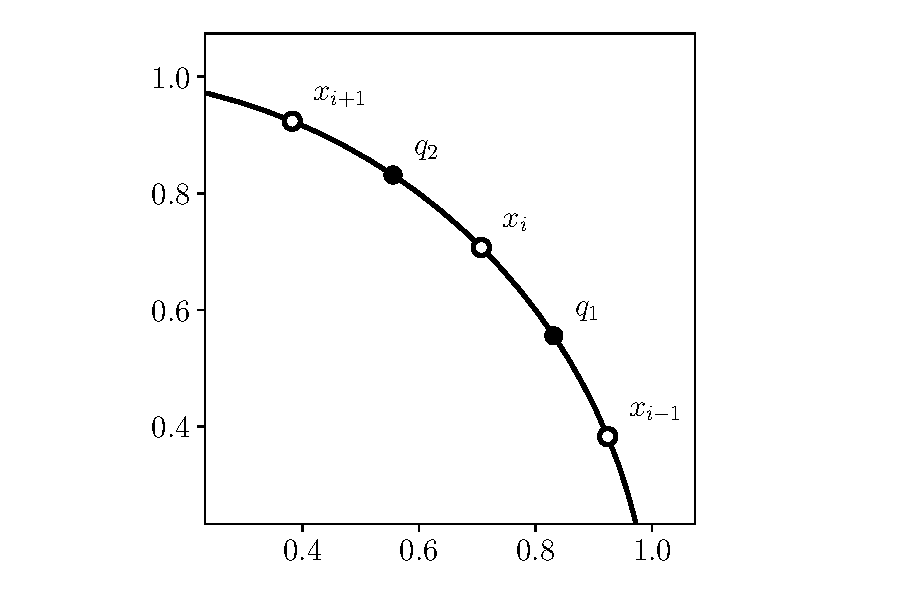
\includegraphics[width=0.8\textwidth]{figures/index.pdf}
    \caption{Bob places two points $q_1$ and $q_2$ in such a way
        on the unit circle, that they can be linearly seperated from the other
        points if and only if Alice didn't place a point at $p_i$.}
    \label{fig:index}
\end{figure}
